\documentclass[a4 paper]{article}
% Set target color model to RGB
\usepackage[inner=2.0cm,outer=2.0cm,top=2.5cm,bottom=2.5cm]{geometry}
\usepackage{setspace}
\usepackage[rgb]{xcolor}
\usepackage{verbatim}
\usepackage{subcaption}
\usepackage{amsgen,amsmath,amstext,amsbsy,amsopn,tikz,amssymb,tkz-linknodes}
\usepackage{fancyhdr}
\usepackage[colorlinks=true, urlcolor=blue,  linkcolor=blue, citecolor=blue]{hyperref}
\usepackage[colorinlistoftodos]{todonotes}
\usepackage{rotating}
\usepackage{listings}
\usepackage[utf8]{inputenc}
\usepackage[portuguese]{babel}
\usepackage{booktabs}

\lstset{language=C,
    upquote=true,
    numbers=left,
    stepnumber=1,
    numbersep=8pt,
    showstringspaces=false,
    breaklines=true,
    frameround=ftff,
    frame=single,
    aboveskip=20pt,
    belowskip=20pt,
}


\title{Sistemas Embarcados - Trabalho Prático 1}
\author{Társio Onofrio Cardoso da Silva}
\date{30 de Maio de 2020}

\begin{document}

\begin{titlepage}
\maketitle
\begin{center}
    Escalonador de tarefas de tempo real utilizando interrupções
\end{center}
\vfill
\noindent Professor: Sergio Johann Filho

\noindent Disciplina: 98G00-04 - Sistemas Embarcados

\noindent Turma:590

\end{titlepage}


\section{Organização}
% como foi organizada (diagramas, módulos, estruturas de dados, etc)
O trabalho está organizado nos arquivos em torna de algumas estruturas de dados e em  três processos: criação, partida e troca de contexto, respectivamente as funções \verb|rt_create|, \verb|rt_start| e \verb|rt_context_switch|. 


\begin{figure}[htp]
    \centering
    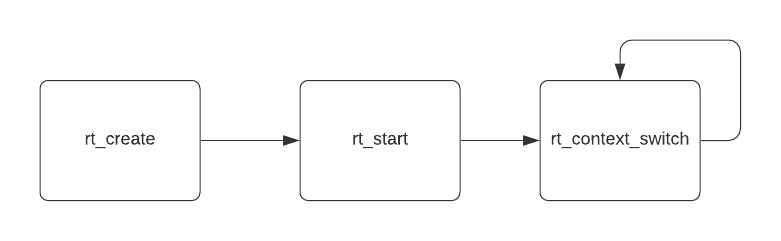
\includegraphics[width=8cm]{process}
    \caption{Processos do sistema}
    \label{fig:process}
\end{figure}

\subsection{Criação}
No processo de criação iniciado pela função \verb|rt_create| é alocado espaço para as lista, a lista das tarefas é inicializada. Após a execução dessa função o usuário pode adicionar tarefas e executar o processo de partida.

\subsection{Partida}
O processo de partida é executado pela função \verb|rt_start|. Nesse processo a tarefa ociosa é criada e as funções de cada tarefa tem seu contexto salvo nos registradores. Ao final deste processo a função \verb|rt_clock| é chamada e a interrupção por cronômetro é definida e ativada, e por fim é chamado um laço infinito.

\subsection{Troca de contexto}
Após a execução do laço infinito iniciam as interrupções  por cronometro, função \verb|timer1ctc_handler|, que chama as trocas de contexto, função \verb|rt_context_switch|, fazendo uso do algoritmo \textit{rate monotonic}. Após definir definir o estado futuro da tarefa em execução, seleciona uma nova tarefa se necessário, ativa novamente as interrupções e pula para a tarefa escolhida. O laço entre \verb|timer1ctc_handler|,  \verb|rt_context_switch| e \verb|rt_task| é repetido infinitamente.

\subsection{Variáveis globais e estruturas de dados}

O escalonador usa algumas variáveis e estruturas de dados para realizar o escalonador de tarefas em tempo real. 

\begin{lstlisting}[captionpos=b, language=C, caption=Estado da tarefa]
enum enum_state{READY,
                RUNNING,
                BLOCKED,
                DONE,
                SYS}
                rt_state;
\end{lstlisting}

A seguir é descrito cada estado:

\begin{itemize}
\item \verb|READY|: tarefas prontas para serem escalonadas;
\item \verb|RUNNING|: tarefa em execução;
\item \verb|BLOCKED|: tarefas bloqueadas pelo sistema, nesse caso nenhuma;
\item \verb|SYS|: tarefas do sistema, nesse caso somente a tarefa de espera(\verb|rt_idle_function|).
\end{itemize}

Os estados de cada tarefa estão são uma das variáveis dentro da estrutura de dados da tarefa, descrita abaixo:

\begin{lstlisting}[captionpos=b, language=C, caption=Estrutura de dados das tarefa, label={lst:rt_task}]
typedef struct{
    void (*_function)();
    int _id;
    char *_name;
    int _period;
    int _capacity;
    int _deadline;
    int state;
    int executed;
} rt_task;

rt_task *rt_running_task;
rt_task *rt_idle_task;
\end{lstlisting}

Abaixo é descrita cada variável da estrutura de dados acima:
\begin{itemize}
\item \verb|void (*_function)()|: função da tarefa, definida pelo usuário;
\item \verb|int _id|: número único de identificação da função definido sequencialmente pelo sistema;
\item \verb|char *_name|: nome da da tarefa; 
\item \verb|int _period|: período da tarefa;
\item \verb|int _capacity|: capacidade ou ou tempo de computação da tarefa;  
\item \verb|int state|: estado da tarefa, definido acima;
\item \verb|int executed|: unidades de tempo executadas pela tarefa.
\end{itemize}


As tarefas criadas pelo usuário são adicionadas em uma estrutura de dados encadeada descrita a seguir:
\begin{lstlisting}[captionpos=b, language=C, caption=Lista encadeada]
struct list {
	void *elem;
	struct list *next;
};

struct list *rt_list_task;
\end{lstlisting}


A variável \verb|int rt_time|  é o contador global da unidade de tempo, ele é incrementado pela função 
\verb|rt_context_switch|.


\section{Instruções e casos de uso}
% como utilizar os mecanismos desenvolvidos
% casos de uso, demonstrando as funcionalidades

O sistema é fácil de usar, requerendo o \textit{GCC} com suporte para arquitetura \textit{RISCV 32 bits}, Apresentamos as 

Primeiramente baixe o repositório (privado no momento) no endereço \textit{https://github.com/tarsioonofrio/hf-risc}, e abra o arquivo  \textit{hf-risc/tp1/app/scheduler.c}. Abaixo é apresentada um pequeno exemplo:

\begin{lstlisting}[captionpos=b, language=C, caption=Função de exemplo]
void f(void){
    volatile char cushion[1000];	/* reserve some stack space */
    cushion[0] = '@';	        	/* don't optimize my cushion away */

    if (!setjmp(rt_jmp[rt_running_id]))
        longjmp(rt_jmp[0], 1);


    while (1) {
        /* thread body */
        printf("task 0...%d\n", rt_running);
    }
}
\end{lstlisting}

Escreva uma função sem parâmetros de entrada e sem retorno, as linhas 1 e 2 são essenciais pois reservam espaço na pilha para essa função e impede que o compilador ao otimizar o código remova o espaço reservado. As linhas 5 e 6 reservam salvam o contexto nos registradores e pulam de volta para a função \verb|rt_start|. Por fim adicione o laço infinito com alguma execução dentro.

\begin{lstlisting}[captionpos=b, language=C, caption=Exemplo de uso]
int main(void){
    rt_create();

    rt_add_task(f, 20, 3, 0, "1", READY);
    rt_add_task(f, 05, 2, 0, "2", READY);
    rt_add_task(f, 10, 2, 0, "3", READY);

    rt_start();
    return 0;
}
\end{lstlisting}

Na função \verb|main| adicione \verb|rt_create| antes de \verb|rt_add_task| que fará a adição das tarefas no escalonador.
\begin{lstlisting}[captionpos=b, language=C, caption=Função de adição das tarefas]
int rt_add_task(void (*function), 
                int period, 
                int capacity, 
                int deadline, 
                char *name,  
                int state);
\end{lstlisting}

Os parâmetros da função \verb|rt_add_task| são praticamente iguais as variáveis descritas em \ref{lst:rt_task}, menos \verb|_id| e \verb|executed|. Após isso basta executar \verb|rt_start|.

Há ainda outras funções que podem ser usadas no sistema:
\begin{itemize}
    \item \verb|const int  rt_get_states()|: retorna os estados de todas as tarefas;
    \item \verb|const int  rt_get_ids()|: retorna os identificadores numéricos de todas as tarefas;
    \item \verb|int rt_del_task(int id)|: remove uma tarefa pelo seu identificador numérico;
    \item \verb|int rt_task_count()|: retorna total de tarefas.
\end{itemize}

\section{Avaliação do custo da implementação}
% avaliação do custo da implementação (tamanho do código para cada subsistema, custo em ciclos do algoritmo de escalonamento, etc).


\end{document} 
